\section{Versuchsdurchführung}
\subsection{Teil I: Pockels-Effekt}
\subsubsection{Bestimmung der Halbwellenspannung mit einer Sägezahnspannung}
Um eine grobe Abschätzung der Halbwellenspannung zu bekommen,
wird im ersten Versuchsteil an die Pockelszelle das Sägezahnsignal angelegt.
Gleichzeitig wird mit dem Oszilloskop das Spannungssignal nach dem Verstärker der Photodiode gemessen.
Durch Drehen des Analysators wird dieses Signal so eingestellt,
dass die Amplitude maximal ist, aber kein \emph{Clipping} auftritt.
Die beiden Signale werden mit dem Computer aufgezeichnet.
Anschließend wird der Analysator für zwei weitere Messungen jeweils ein wenig weiter verdreht,
um eine eventuelle Amplitudenabhängigkeit der Halbwellenspannung zu identifizieren. 


\subsubsection{Bestimmung der Halbwellenspannung durch Periodenverdopplung eines Wechselsignals}

\paragraph{Ursache der Periodenverdopplung}
In diesem Versuchsteil wird die Halbwellenspannung mit einer genaueren Messmethode bestimmt:
Wenn ein Wechselsignal einer Gleichspannung überlagert wird,
dann verdoppelt die Wechselspannung ihre Frequenz,
wenn der Wert der Gleichspannung ein Vielfaches der Halbwellenspannung beträgt.
Die Ursache davon wird im Folgenden erläutert.\\
Die winkelabhängige Transmission des Analysators wird durch das Gesetz von Malus beschrieben:
Linear polarisiertes Licht, dessen Polarisationsrichtung um den Winkel $\alpha$ zur Achse des Analysators
gedreht ist, wird mit dem Faktor $\cos^2(\alpha)$ abgeschwächt.
Ist die Analysatorachse parallel zur Polarisatorachse vor der Pockelszelle eingestellt,
gilt (da bei Halbwellenspannung die Polarisation um 90$^\circ$ gedreht wird)
folgende Abhängigkeit des Winkels $\alpha$ von der Spannung $U$ an der Pockelszelle
und der Halbwellenspannung $U_{\lambda / 2}$:
\begin{equation}
\label{}
  \alpha = \frac{\pi}{2} \cdot \frac{U}{U_{\lambda / 2}}
\end{equation}
Daraus folgt für die Intensität $I$ nach dem Analysator
\begin{equation}
\label{eq:int}
  \frac{I}{I_0}=\cos^2(\frac{\pi}{2} \cdot \frac{U}{U_{\lambda / 2}})
\end{equation}
$I_0$ ist die Lichtintensität vor dem Analysator. Der Zusammenhang ist auf \autoref{img:pocktheo1}
für $U_{\lambda / 2}=221\,$V dargestellt.

\begin{figure}[H]
\begin{center}
  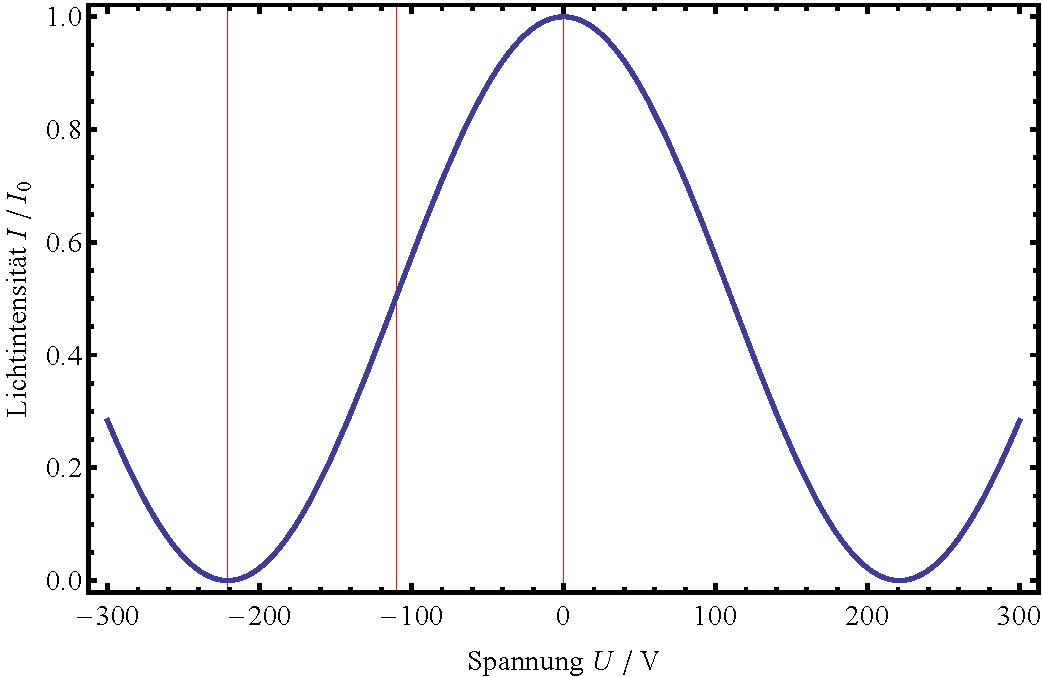
\includegraphics[width=0.7\textwidth]{../img/Pocktheo1.pdf}
  \caption{Lichtintensität nach dem Analysator in Abhängigkeit der Spannung an der Pockelszelle.
  Die roten Linien zeigt die drei Gleichspannungen, denen auf \autoref{img:pocktheo2} ein Wechselsignal
  überlagert ist.}
  \label{img:pocktheo1}
\end{center}
\end{figure}

Besteht die Spannung $U$ aus dem Gleichanteil $U_\text{G}$ und dem Wechselanteil
\mbox{$U_\text{W}=A\sin(\omega t)$}
mit der Kreisfrequenz $\omega$,
so gilt für die zeitabhängige Abschwächung durch den Analysator
\begin{equation}
\label{eq:intt}
  \frac{I}{I_0}(t)=\cos^2(\frac{\pi}{2} \cdot \frac{U_\text{G} + A\cdot\sin(\omega t)}{U_{\lambda / 2}})
\end{equation}
\autoref{img:pocktheo2} zeigt diese Zeitabhängigkeit für verschiedene Gleichanteile,
\mbox{$A=30$\,V} und $\omega=1$\,kHz.\\
Wenn der Gleichanteil so eingestellt wird,
dass eine mittelhohe Intensität durch den Analysator transmittiert wird,
so wird das Wechselsignal fast unverformt übertragen.
Dies gilt aber nicht mehr, wenn der Gleichanteil so eingestellt ist,
dass ein Transmissionsmaximum oder -minimum auftritt.
Dann oszilliert das Wechselsignal um diesen Extrempunkt auf \autoref{img:pocktheo1}.
Pro Schwingungsperiode des Wechselsignals wird somit zweimal ein Intensitätsminimum bzw. -maximum erreicht:
Periodenverdoppelung tritt auf.\\
Der Einsatz der Periodenverdopplung kann auf \autoref{img:pocktheo3} abgelesen werden:
Hier ist die Intensität in Abhängigkeit der Zeit und der Gleichspannung gezeigt.
Die Periodenverdoppelung tritt auch schon weiter entfernt von den Extrema auf,
hier erhält man aber kein symmetrische Signal.\\
Die Beobachtung des Signals der Photodiode liefert also ein sehr gutes Kriterium zur
Bestimmung der Halbwellenspannung:
Misst man ein symmetrisches Signal mit doppelter Anregungsfrequenz,
dann ist die Gleichspannung so eingestellt,
dass die Transmission minimal oder maximal ist.
Die Differenz von zwei Spannungswerten bei Minimum und Maximum ist die Halbwellenspannung.

\begin{figure}[H]
\begin{center}
  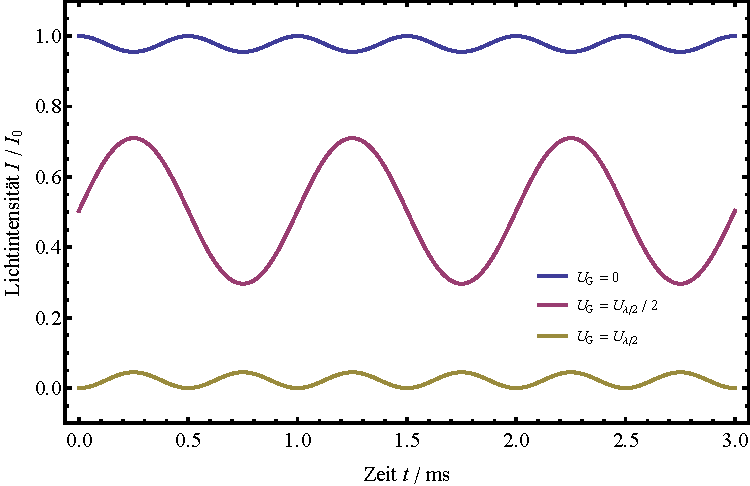
\includegraphics[width=0.7\textwidth]{../img/Pocktheo2.pdf}
  \caption{Zeitabhängigkeit der Intensität nach dem Analysator für verschiedene Gleichanteile $U_\text{G}$
  nach \autoref{eq:intt} für $\omega=1$\,kHz und $A=30$\,V.
  Die $U_\text{G}$ sind auf \autoref{img:pocktheo2} eingetragen.}
  \label{img:pocktheo2}
\end{center}
\end{figure}

\begin{figure}[H]
\begin{center}
  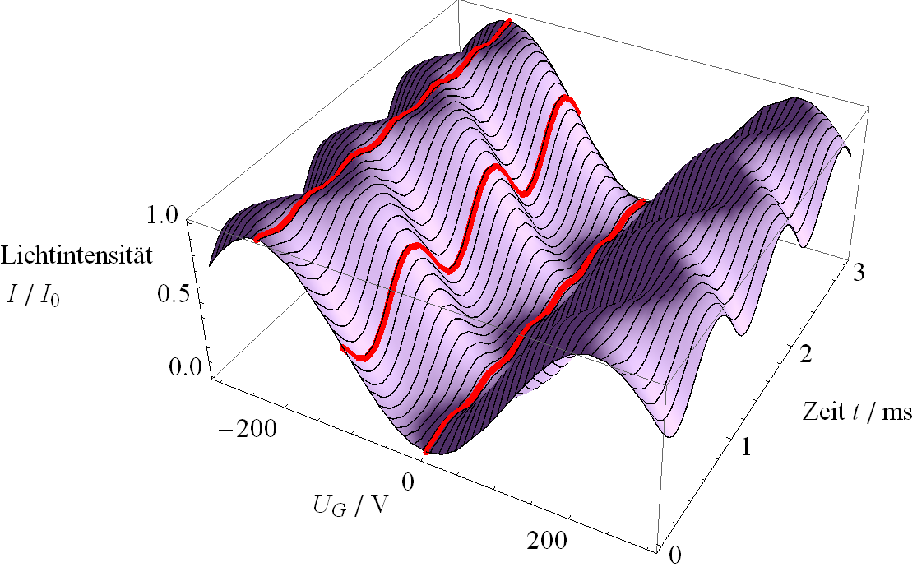
\includegraphics[width=0.88\textwidth]{../img/Pocktheo3.pdf}
  \caption{Zeitliche Variation der Intensität nach dem Analysator
  in Abhängigkeit des Gleichanteils $U_{\text{G}}$ der Spannung an der Pockelszelle nach \autoref{eq:intt}.
  Die roten Linien sind die Kurven aus \autoref{img:pocktheo2}.
  Es ist erkennbar, dass im Bereich um die Extrema eine Periodenverdoppelung des Wechselsignals auftritt.}
  \label{img:pocktheo3}
\end{center}
\end{figure}

\paragraph{Einfluss des Umgebungslichts auf die Messung}
Wenn die Messung so durchgeführt wird, wie oben beschrieben,
müssen die Signale auf dem Oszilloskop sehr genau beobachtet werden,
um die richtige Einstellung des Gleichanteils $U_{\text{G}}$ zu finden.
Dabei fiel auf, dass an dem Messaufbau ein großes Störsignal durch die Raumbeleuchtung
mit Leuchtstoffröhren auftritt.
\autoref{img:licht} zeigt das Signal der Photodiode bei ausgeschaltetem Laser (gelbe Kurve),
wenn das Raumlicht ungehindert auf sie fällt.
Mit einer Papierröhre um den Strahlengang vor der Diode und einem
dunklen Tuch als Abschirmung konnte das Störsignal fast vollständig unterdrückt werden (orange und rot).
Bei ausgeschaltetem Raumlicht verschwindet das Störsignal vollständig (schwarz).\\
Das Störsignal hat die doppelte Netzfrequenz (100\,Hz), weil die Leuchtstoffröhren bei Maximum und
Minimum des Netzsignals hell leuchten und bei jedem Nulldurchgang dunkel sind.

\begin{figure}[H]
\begin{center}
  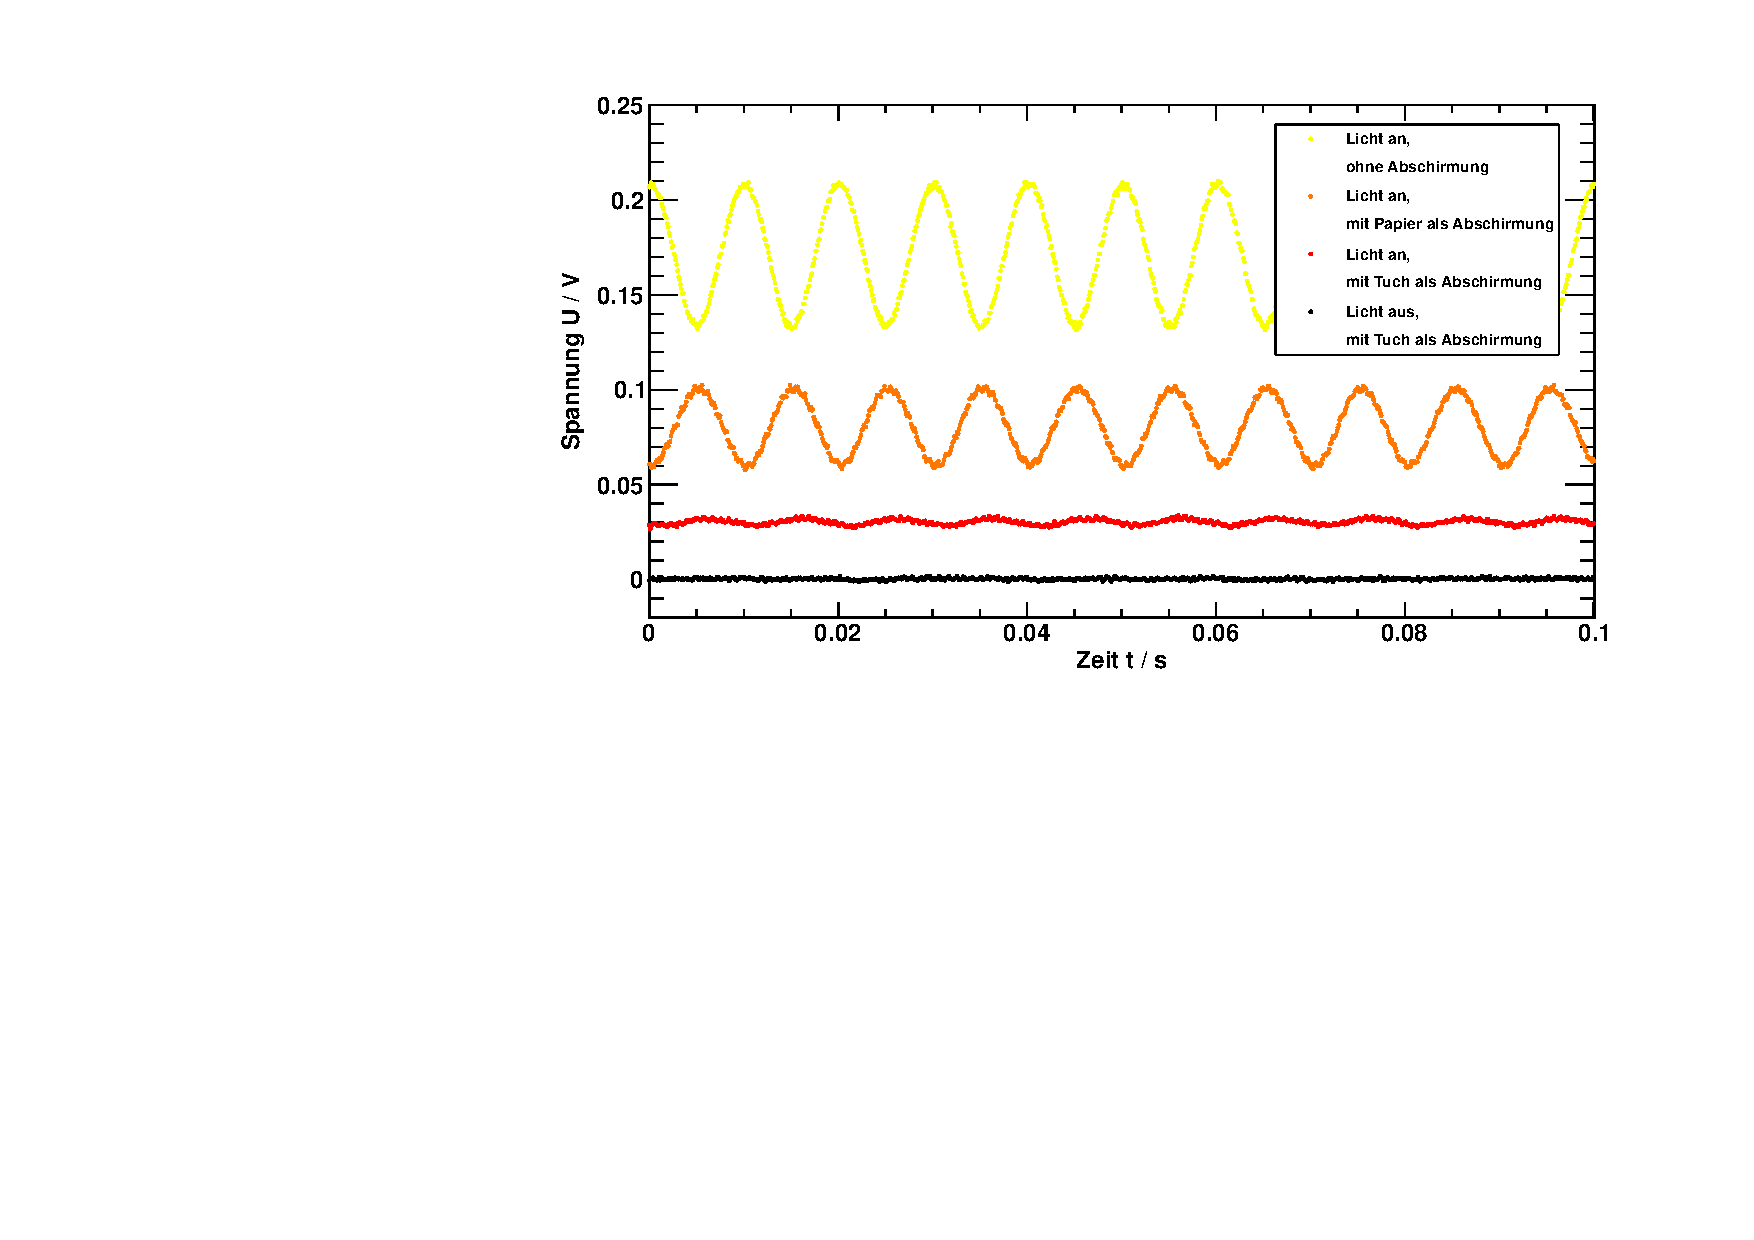
\includegraphics[width=0.9\textwidth]{../img/licht.pdf}
  \caption{Störsignal mit Frequenz 100\,Hz durch die Neonlampen an der Decke des Labors und
  Beseitigung durch geeignete Abschirmung.
  Zur besseren Übersicht wurden die drei oberen Signale mit Offset eingezeichnet. }
  \label{img:licht}
\end{center}
\end{figure}


\paragraph{Durchführung}
Es werden nun zwei Messreihen bei unterschiedlichen Frequenzen des Sinussignals durchgeführt
($\omega_1=1$\,kHz und $\omega_2=10$\,kHz).
Die Amplitude des Wechselsignals wird mit dem Oszilloskop gemessen und beträgt dort
$A=125$\,mV. Wenn man von einem Verstärkungsfaktor von ungefähr 100 ausgeht,
liegt an der Pockelszelle also eine Sinusspannung mit der Amplitude $A'=12.5$\,V an.
Diesem Sinussignal ist die Gleichspannung $U_{\text{G}}$ überlagert,
die so eingestellt wird, dass am Oszilloskop ein symmetrisches Photodiodensignal sichtbar ist.
\autoref{img:pockdurchf} zeigt diesen Vorgang.

Für beide Frequenzen wurde am Transmissionsmaximum und -minimum
die notwendige Gleichspannung für ein symmetrisches
Photodiodensignal eingestellt und die Spannung $U_{\text{G}}$ notiert.

\begin{figure}[H]
\begin{center}
  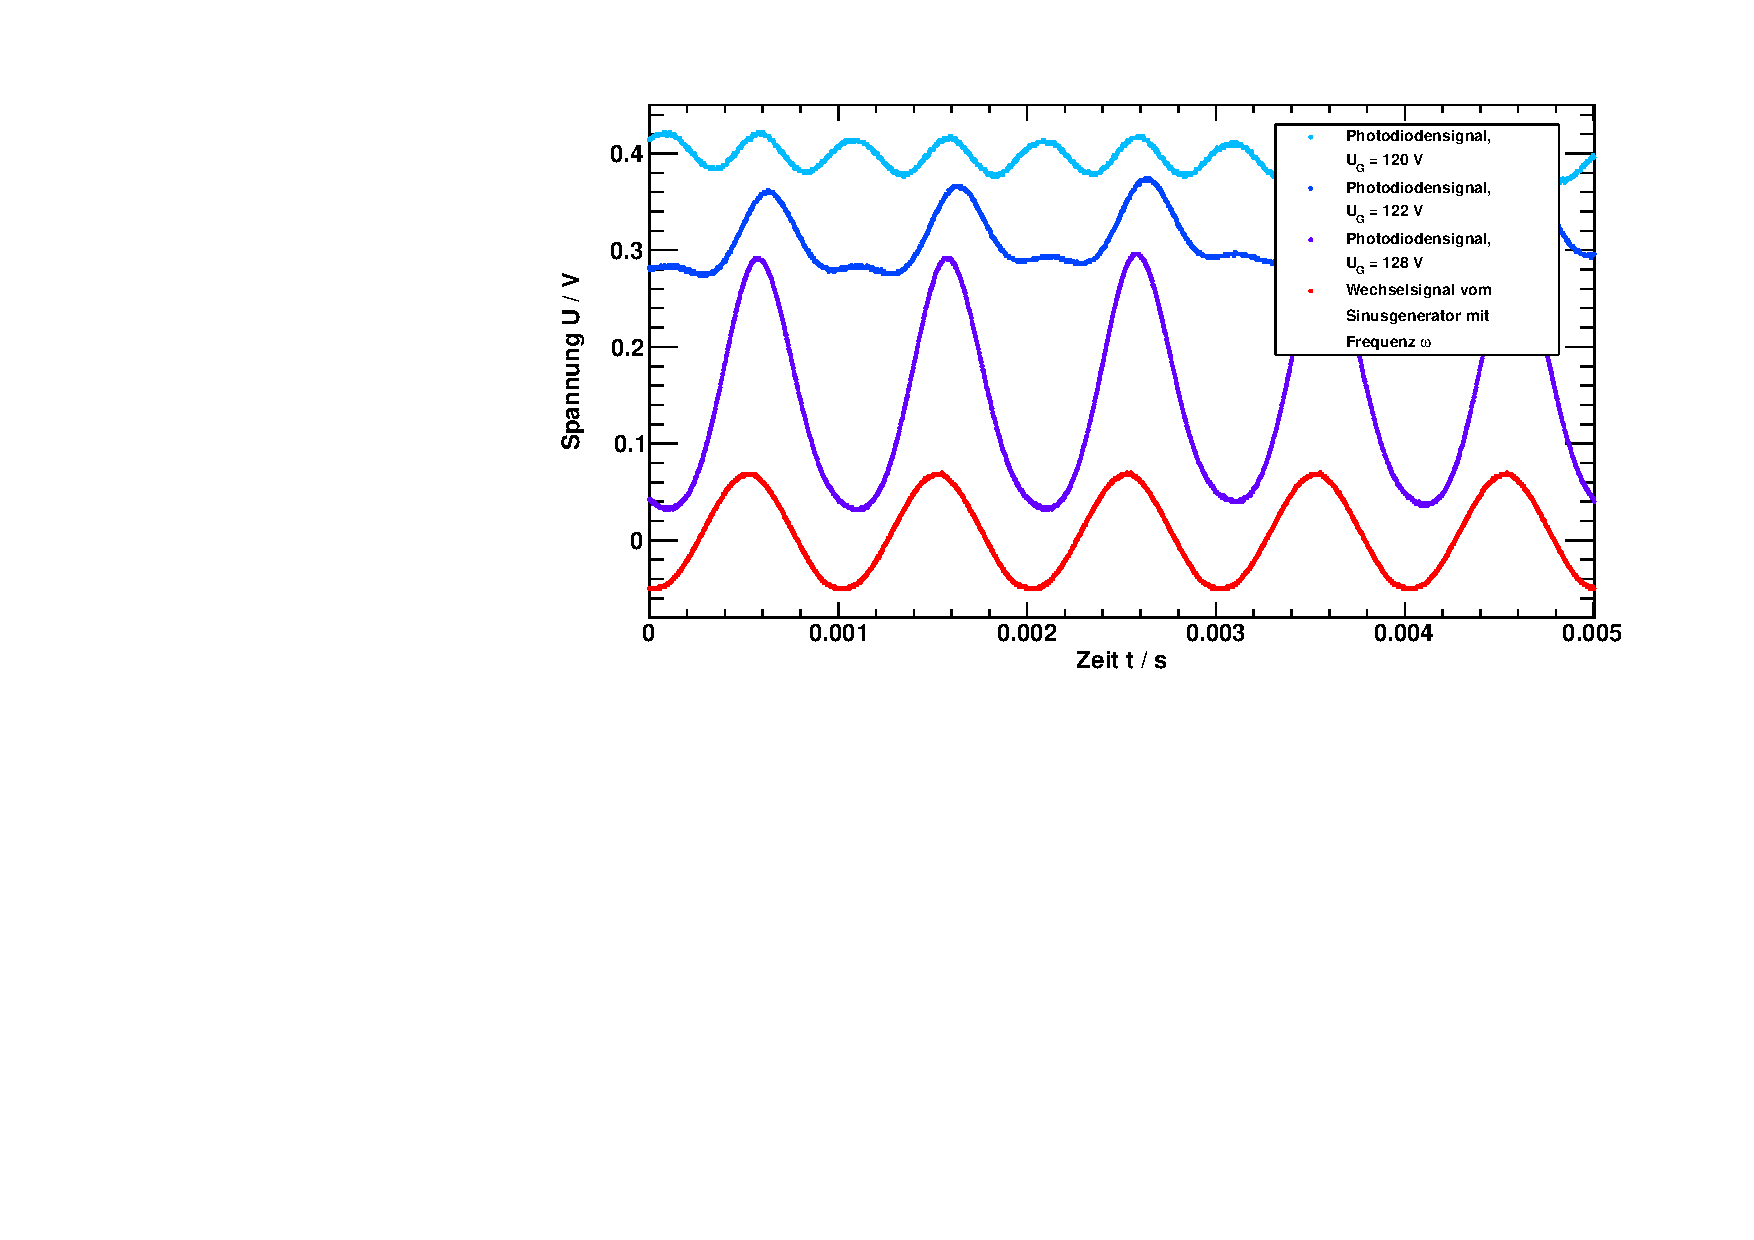
\includegraphics[width=0.9\textwidth]{../img/pockdurchf.pdf}
  \caption{Photodiodensignale, die durch Änderung der Gleichspannung $U_\text{G}$
  bei der Suche nach dem periodenverdoppelten Signal auftreten.
  Eine Abweichung um 2\,V vom optimalen Wert bei $U_\text{G}=120$\,V ist bereits deutlich 
  an der asymmetrischen Signalform sichtbar.}
  \label{img:pockdurchf}
\end{center}
\end{figure}


\subsection{Teil II: Faraday-Effekt}
-erwähne Messreihenfolge --> Aufspüren systematischer Fehler \\
-Bild für verschiedene Einstellungen von Halbschattenpolarimeter